\section{Reservas Bancarias y Riesgo Crédito}
%\index{Reservas Bancarias y Riesgo Crédito}
\subsection{El papel de las reservas bancarias en la estabilidad financiera y la gestión de riesgos}
%\index{Las reservas bancarias en riesgos}
Las reservas bancarias tienen un papel fundamental en la estabilidad financiera y  la gestión de riesgos del sistema bancario. Las reservas son esenciales para afrontar demandas de liquidez asegurando la continuidad operativa de los bancos. Desde el punto de vista de la política monetaria, el nivel de reservas bancarias es una herramienta utilizada por los bancos centrales para influir en la oferta monetaria, las tasas de interés y, por ende, en variables macroeconómicas claves como la inflación y el crecimiento económico.
Si centramos el foco en analizar las reservas desde un punto de vista de la relación entre estas y la probabilidad de quiebra bancaria, podemos afirmar que cuando el ajuste de las tasas no es del todo correcto, el efecto de costo derivado de mayores requisitos de reserva puede incentivar a los bancos a elegir activos más riesgosos.\footnote{C. Glocker (2021). Reserve requirements and financial stability.} Desde el punto de vista de las instituciones bancarias, es bastante fácil ver que el tener pocas reservas podría provocar que una institución sea más propensa a la crisis, pero un exceso de reservas puede llevar a perder rentabilidad. Por otro lado, si ahora ponemos el foco en la relación entre el créditohabiente y la institución bancaria, es fácil notar que precios muy altos para los créditos podrían llevar a los créditohabientes a una saturación excesiva y por tanto, aumentar su riesgo de mora, pero precios muy bajos, podrían provocar que la institución bancaria pierda rentabilidad o bien, le sea muy difícil cumplir con sus obligaciones de reserva por créditos. Por tanto, podemos identificar un problema de equilibrio en el establecimiento de precios para créditos, siempre bajo la óptica de la correcta constitución de reservas. 


\subsection{Análisis de las Reservas Bancarias en Guatemala }
%\index{Análisis de las Reservas Bancarias en Guatemala}
En la siguiente gráfica podemos apreciar la evolución de la constitución de reservas en Guatemala desde enero de 2018 a febrero de 2024. 
\begin{figure}[h]
    \centering
    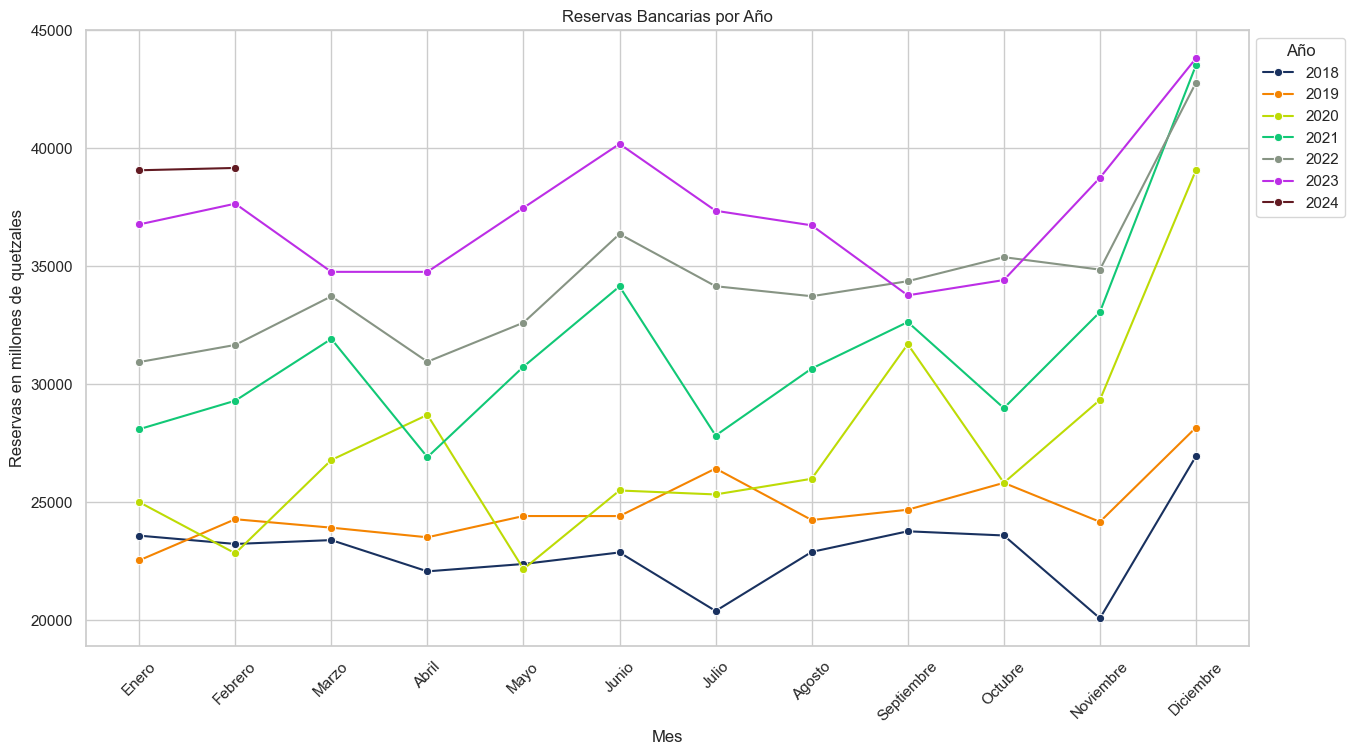
\includegraphics[scale=0.5]{imagenes/reservas_en_guatemala.png}
    \caption{Evolución de la constitución de reservas bancarias en Guatemala.}
    \small{Fuente: Elaboración propia a partir de  datos del Banco de Guatemala.}
    \label{evolucion de reservas}
\end{figure}

%agregar variaciones intermensiales, interanuales y analizar algo de la tendencia


A simple vista, lo primero que podríamos decir es que, en promedio, las reservas bancarias tienden a incrementarse con el tiempo. Por otro lado, es importante resaltar que no hay ningún año en el que las reservas de cualquier mes caigan por debajo del mínimo registrado en los años anteriores. Aun así, sí es posible identificar que, en determinados meses, las reservas son inferiores a las reservas máximas alcanzadas en algún punto de años previos. Esto nos lleva a concluir que aunque las reservas muestran un incremento al concluir cada año, hay momentos específicos dentro del año en los que las reservas bancarias no alcanzan algunos valores observados en periodos previos. Por ejemplo, podemos observar que los valores mínimos de las reservas en 2019, 2020 y 2021 son menores que los máximos registrados en todos los años analizados antes. Los años 2022 y 2023 presentan esta tendencia de manera parcialmente, por lo que, aunque la tendencia no se ha eliminado por completo, parece observarse cierta mejora. \\



Por otro lado, hay que considerar que una perspectiva importante a contemplar es la relación entre las reservas bancarias y la inflación. Se sabe que el aumentar el porcentaje de reservas requeridas puede conllevar a una disminución de los recursos líquidos que las instituciones financieras poseen para la concesión de créditos, induciendo una contracción en la masa monetaria circulante dentro de la economía. Por otro lado, al disminuir el porcentaje,los bancos pueden prestar más, lo que potencialmente provoca una alza en la inflación. Con el fin de analizar las reservas bancarias y la inflación en Guatemala, a continuación un análisis de las variaciones intermensuales absolutas y la evolución de la constitución de reservas en relación con la inflación mensual. 


\subsubsection{Variaciones Intermensuales e Interanuales Absolutas}
En este apartado haremos un análisis descriptivo breve y general de la constitución de reservas en Guatemala en los últimos años y los meses transcurridos del 2024. Comenzaremos por examinar las variaciones interanuales absolutas para luego abordar las variaciones intermensuales absolutas. Posteriormente, buscaremos comparar la constitución de reservas con la dinámica inflacionaria del país, con el objetivo de evaluar cómo ha evolucionado el valor real de las reservas bancarias a lo largo del tiempo y qué efecto ha tenido la inflación sobre las reservas.
\newpage
\begin{figure}[ht!]
    \begin{minipage}{0.5\textwidth}
        \centering
        \begin{center}
Variaciones Interanuales Absolutas en la \\ 
Reserva Bancaria Nacional  en Diciembre \\
de cada año en millones de quetzales\\
\begin{tabular}{
  @{}
  l % Columna de año como texto (o entero sin formato especial de siunitx)
  S[table-format=4.0] % Esto no debería aplicarse a la columna de años; ajuste hecho en la siguiente línea
  S[table-format=-5.1] % Columna de variación con formato numérico
  @{}
}
\toprule
\textbf{{Año}} & \textbf{{Variación}} \\
\midrule
2019 & 1215.3 \\
2020 & 10913.3 \\
2021 & 4448.1 \\
2022 & -740.2 \\
2023 & 1031.4 \\
\bottomrule
\end{tabular}
\end{center}
    \end{minipage}%
    \begin{minipage}{0.5\textwidth}
        Una observación clara y directa es que, entre los últimos seis años, el 2022 destaca por ser el único en registrar una disminución absoluta en la formación de reservas bancarias. Adicionalmente, es notable que la variación en 2020 superó la suma total de las variaciones de los demás años combinados.
    \end{minipage}
\end{figure}
La siguiente tabla muestra las variaciones intermensuales absolutas en la Reserva Nacional Bancaria de Guatemala
\begin{table}[H]
\begin{center}
Variaciones Intermensuales Absolutas en la Reserva Bancaria Nacional \\
de Guatemala en millones de quetzales \footnote{Diferencias intermensuales absolutas en las reservas bancarias en Guatemala.}
\\
\begin{tabular}{
  @{}
  l
  S[table-format=-4.1]
  S[table-format=-4.1]
  S[table-format=-4.1]
  S[table-format=-4.1]
  S[table-format=-4.1]
  S[table-format=-4.1]
  @{}
}
\toprule
\textbf{Mes} & {\textbf{2018}} & {\textbf{2019}} & {\textbf{2020}} & {\textbf{2021}} & {\textbf{2022}} & {\textbf{2023}} \\
\midrule
Ene & 0.0 & -4417.0 & -3162.5 & -10985.4 & -12586.4 & -6011.4 \\
Feb & -352.5 & 1744.7 & -2170.9 & 1208.7 & 725.8 & 879.0 \\
Mar & 163.4 & -357.9 & 3956.4 & 2620.0 & 2060.4 & -2889.7 \\
Abr & -1325.1 & -408.5 & 1913.1 & -5012.1 & -2772.1 & 0.0 \\
May & 312.4 & 901.6 & -6535.6 & 3834.6 & 1655.9 & 2714.6 \\
Jun & 489.8 & -1.8 & 3329.5 & 3402.1 & 3757.9 & 2708.7 \\
Jul & -2481.9 & 2016.6 & -166.8 & -6321.5 & -2213.5 & -2833.8 \\
Ago & 2504.4 & -2184.2 & 664.1 & 2841.0 & -423.7 & -617.8 \\
Sep & 873.8 & 436.8 & 5704.6 & 1971.0 & 636.6 & -2967.4 \\
Oct & -176.9 & 1139.6 & -5874.4 & -3648.9 & 1019.2 & 648.4 \\
Nov & -3510.9 & -1652.2 & 3511.7 & 4071.5 & -527.8 & 4334.7 \\
Dic & 6871.8 & 3997.6 & 9744.1 & 10467.1 & 7927.5 & 5066.1 \\
\bottomrule
\end{tabular}
\end{center}
\caption{Variaciones Intermensuales Absolutas en la Reserva Bancaria Nacional}
\end{table} 
Podemos observar que el 2021 fue el año con el mayor número de variaciones intermensuales positivas. Asimismo, se observa una reducción significativa de las reservas en enero de cada año. Aunque el país incrementa sus reservas en diciembre, la disminución experimentada en enero excede al incremento de diciembre en el 40\% de los casos analizados.\footnote{Esto corresponde a los años 2021 y 2022.} \\


Finalmente, siguiendo en la línea del análisis general de la constitución de reservas en el país, retomamos el gráfico \ref{evolucion de reservas}, pero le incorporamos un nuevo elemento: partiendo de las reservas al inicio de cada año y tomando en cuenta la inflación mensual del país, proyectamos cómo se habrían mantenido constantes, en términos de valor, las reservas a lo largo del año. Esto permite evaluar el valor de las reservas iniciales, y ver si su valor permanece, al menos inalterado, ante la inflación.  Para cada año, elaboramos un gráfico que ilustra dos curvas: la trayectoria real de las reservas bancarias y la proyección ajustada por la inflación de las reservas para reflejar un valor constante. Al ajustar por inflación, podemos evaluar de manera efectiva el poder adquisitivo de las reservas bancarias y cómo este se ha mantenido o variado.

%Posteriormente, en otro análisis que presentamos, retomando los datos de las reservas bancarias mensuales, procedemos a analizar la evolución de estas  ajustadas por inflación. Para cada año bajo, trazamos una curva que refleja la evolución de las reservas después de descontar el impacto de la inflación mensual. Este enfoque nos permite observar la trayectoria de las reservas de una forma más precisa sobre el verdadero valor de las reservas a lo largo del tiempo. 
El  escenario  se enfoca en mantener constante el valor real de las reservas a través del tiempo, compensando la inflación, por lo que se se fija el monto de reservas de enero de cada año y se hace una proyección del monto en quetzales que tiene el mismo valor en cada uno de los próximos meses. En el gráfico \ref{proyeccion reservas inicio de año}, podemos notar que, en términos de valor, cada año se observó un incremento en las reservas comparado con el mes de enero. El año 2018 se caracterizó por tener, excepto diciembre, un valor de reserva inferior al observado en enero. Por el contrario, en 2019, el valor de la reserva superó al de enero durante todos los meses. Los años subsiguientes mostraron una variabilidad en la que, en algunos meses, el valor de las reservas superó al de inicio de año, mientras que en otros meses, disminuyó. Los años 2020 y 2021 se distinguieron por tener una tasa de inflación más baja en comparación con otros períodos; en 2021 fue positiva en todos los meses, a diferencia de otros años donde se registró deflación en algunos meses.

\begin{figure}[H]
  \centering
  \captionsetup{justification=centering}

  % Fila 1
  \begin{subfigure}[b]{0.495\textwidth}
    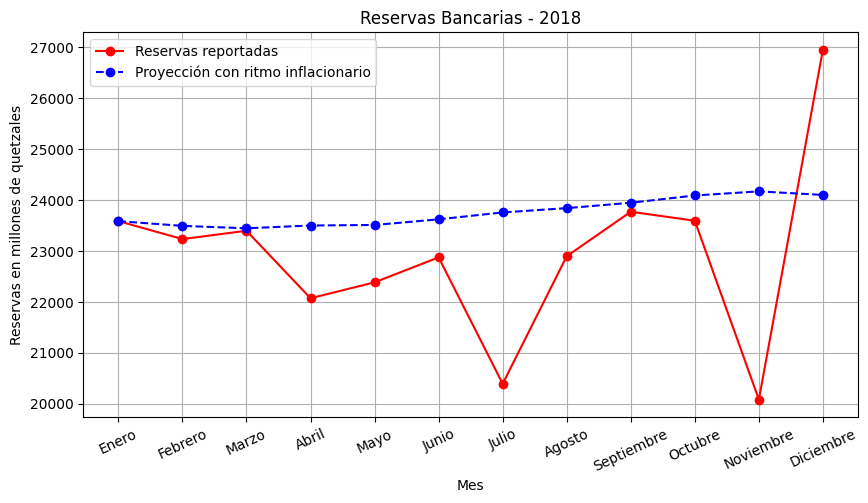
\includegraphics[width=\linewidth]{imagenes/reservas_2018.png}
    \caption{2018}
    \label{proyeccion reservas inicio de año}
  \end{subfigure}
  % No hay espacio intencionalmente entre las figuras para maximizar el tamaño de la imagen
  \begin{subfigure}[b]{0.495\textwidth}
    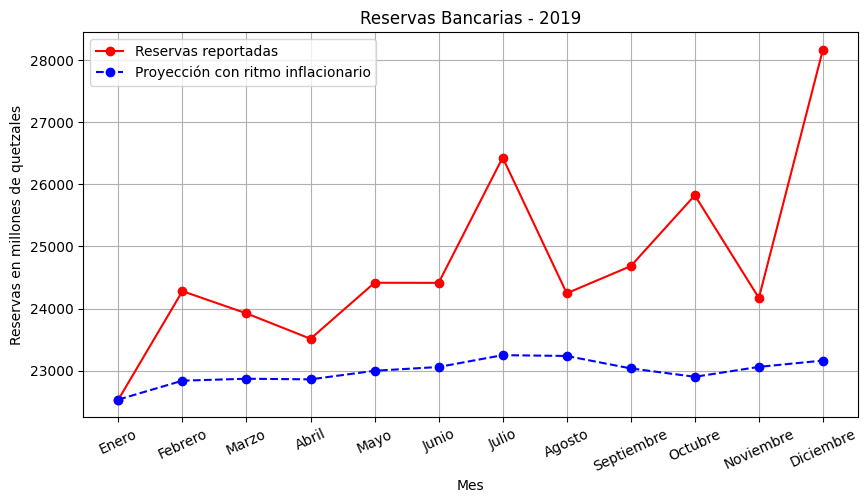
\includegraphics[width=\linewidth]{imagenes/reservas_2019.png}
    \caption{2019}
  \end{subfigure}
  
  % Fila 2
  \begin{subfigure}[b]{0.495\textwidth}
    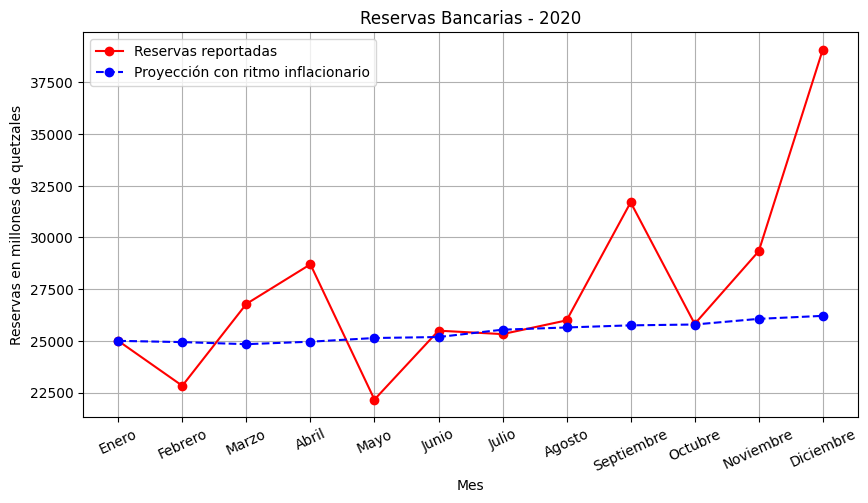
\includegraphics[width=\linewidth]{imagenes/reservas_2020.png}
    \caption{2020}
  \end{subfigure}
  % No hay espacio intencionalmente entre las figuras para maximizar el tamaño de la imagen
  \begin{subfigure}[b]{0.495\textwidth}
    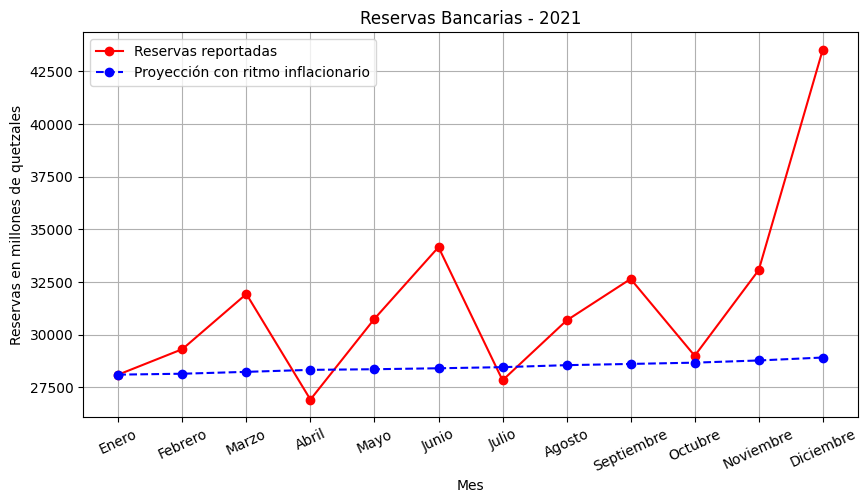
\includegraphics[width=\linewidth]{imagenes/reservas_2021.png}
    \caption{2021}
  \end{subfigure}
  
  % Fila 3
  \begin{subfigure}[b]{0.495\textwidth}
    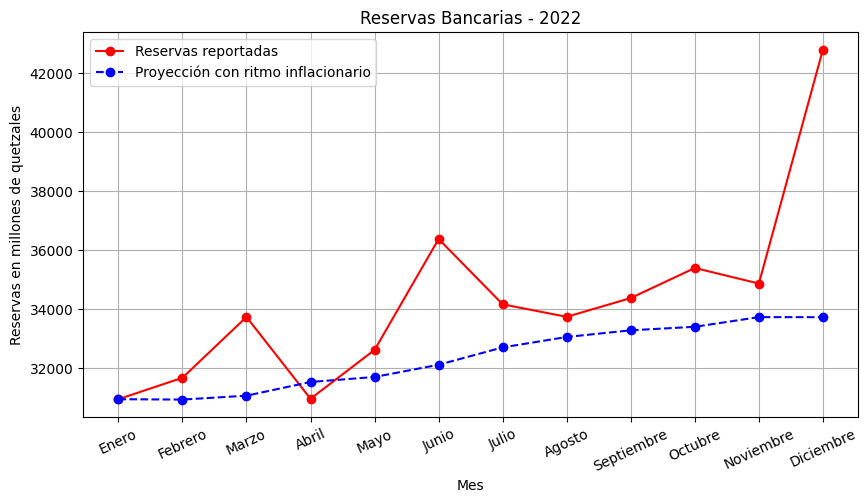
\includegraphics[width=\linewidth]{imagenes/reservas_2022.png}
    \caption{2022}
  \end{subfigure}
  % No hay espacio intencionalmente entre las figuras para maximizar el tamaño de la imagen
  \begin{subfigure}[b]{0.495\textwidth}
    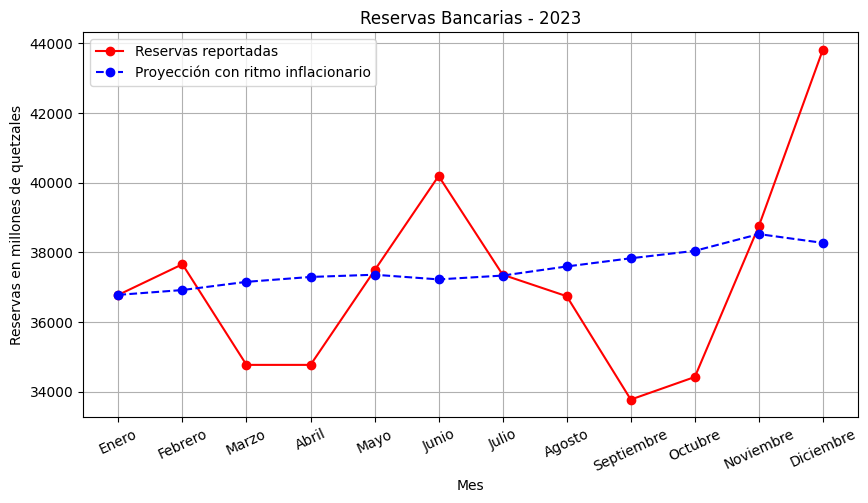
\includegraphics[width=\linewidth]{imagenes/reservas_2023.png}
    \caption{2023}
  \end{subfigure}
\caption{Proyección de valor constante de las Reservas a inicio de año bajo efecto de la inflación}
\end{figure}
\newpage
Observamos que las reservas proyectadas, que se ajustan por inflación de manera progresiva mes a mes, generalmente están por debajo de las reservas reales reportadas. Esto indica que las reservas bancarias no solo han crecido lo suficiente para contrarrestar la inflación, sino que han aumentado en términos de poder adquisitivo.


%En el segundo análisis, en vez de fijar el valor en quetzales de las reservas de enero de cada año, fijamos el valor del dinero en enero de cada año y hacemos una proyección del equivalente en quetzales a las reservas constituidas cada mes según la métrica de valor del dinero de inicio de ese año. Tomando el gráfico \ref{evolucion de reservas}, trazamos la nueva curva para la comparación. Obtenemos las gráficas  \ref{proyeccion retro}.

%Al ajustar las reservas reportadas mes a mes, eliminando el efecto de la inflación, buscamos evaluar cómo se hubieran comportado las reservas si se hubiera reservado lo mismo en valor, y no hubiese existido el efecto de la inflación. Podemos observar, como era de esperarse, que el efecto de la inflación\footnote{Datos de inflación recuperados del Instituto Nacional de Estadística} provocó una desaceleración, en muchos casos, del valor adquisitivo de las reservas. Los años 

%Podemos observar que en ciertos puntos  el poder adquisitivo real de las reservas parece disminuir con el tiempo (esto es claro en los puntos en los que la curva \textcolor{red}{roja} está por debajo de la curva \textcolor{blue}{azul}. Los años 2019, 2021 y 2022 destacan por estar, en la mayoría de meses del año, en temas de consitución de reservas, por encima de las reservas en quetzales requeridas para igualar al valor de las reservas de inicio de año. Es decir, durante la mayoría de los meses de esos años, el valor de las reservas aumentó respecto de inicio de año. Por otro lado, en 2018 podemos observar que solamente en septiembre, octubre y diciembre, las reservas crecieron en valor respecto de enero. Los años 2020 y 2023 tienen un comportamiento más fluctuante en cuanto al crecimiento en valor. En general, el lector podrá notar que estas proyecciones se asemejan mucho a las realizadas en el primer análisis. Esto ocurre pues la perspectiva de ambos análisis fue evaluar la constitución de reservas bajo la óptica de la situación a inicio de cada año, siendo en el primer análisis, una comparativa entre el dinero guardado y el dinero necesario a guardar para mantener el valor de enero, mientras que en el segundo, una evaluación del impacto de la inflación en cada mes.

%\begin{figure}[H]
  \centering
  \captionsetup{justification=centering}

  % Fila 1
  \begin{subfigure}[b]{0.495\textwidth}
    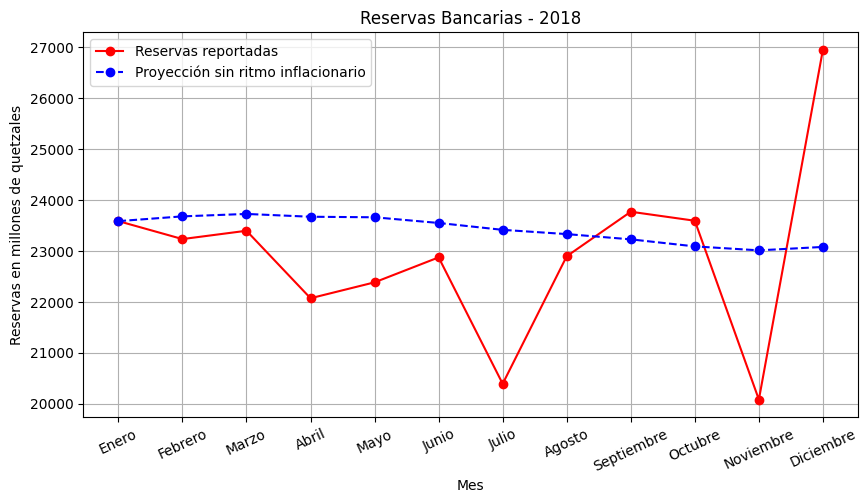
\includegraphics[width=\linewidth]{imagenes/retro_2018.png}
    \caption{2018}
    \label{proyeccion retro}
  \end{subfigure}
  % No hay espacio intencionalmente entre las figuras para maximizar el tamaño de la imagen
  \begin{subfigure}[b]{0.495\textwidth}
    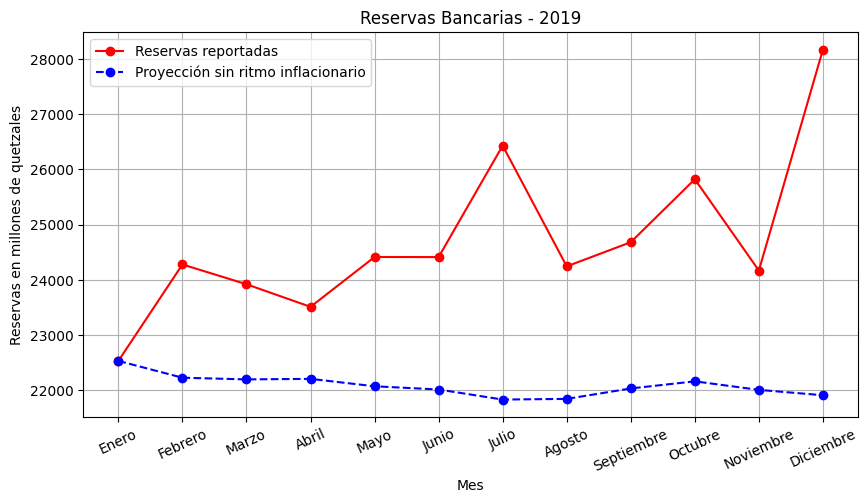
\includegraphics[width=\linewidth]{imagenes/retro_2019.png}
    \caption{2019}
  \end{subfigure}
  
  % Fila 2
  \begin{subfigure}[b]{0.495\textwidth}
    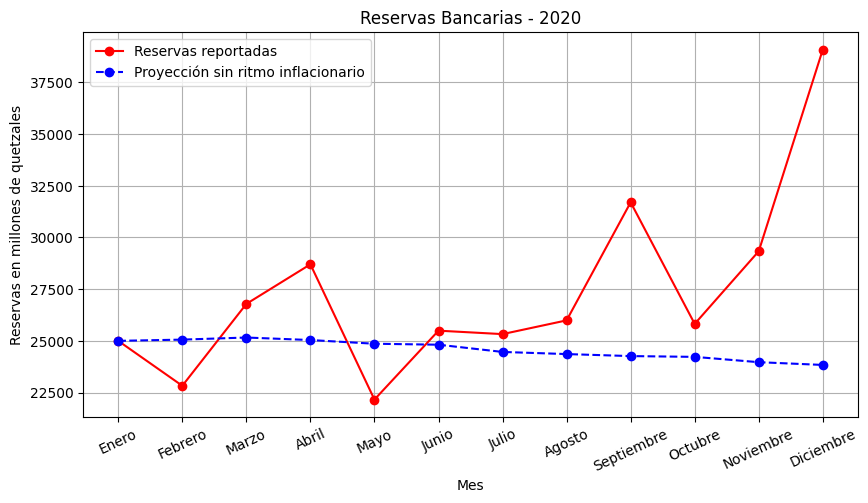
\includegraphics[width=\linewidth]{imagenes/retro_2020.png}
    \caption{2020}
  \end{subfigure}
  % No hay espacio intencionalmente entre las figuras para maximizar el tamaño de la imagen
  \begin{subfigure}[b]{0.495\textwidth}
    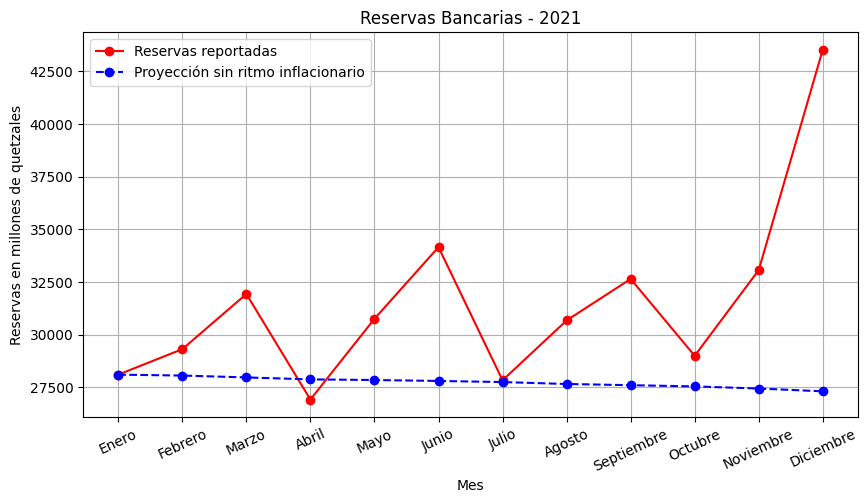
\includegraphics[width=\linewidth]{imagenes/retro_2021.png}
    \caption{2021}
  \end{subfigure}
  
  % Fila 3
  \begin{subfigure}[b]{0.495\textwidth}
    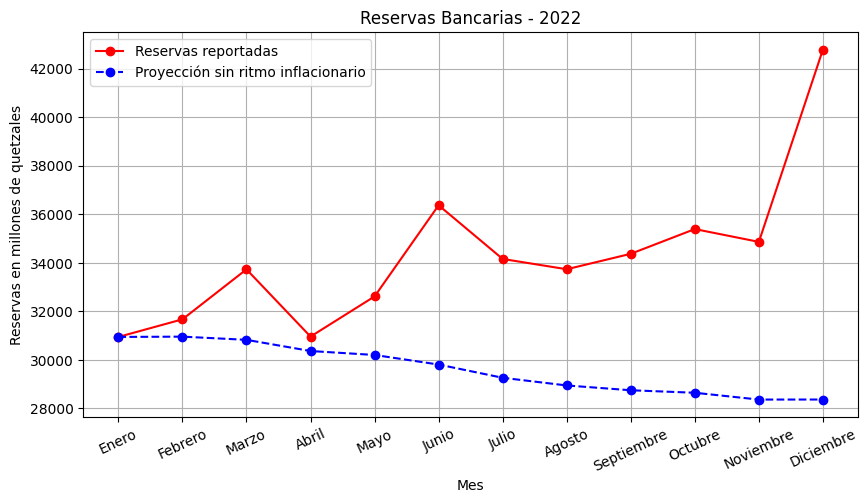
\includegraphics[width=\linewidth]{imagenes/retro_2022.png}
    \caption{2022}
  \end{subfigure}
  % No hay espacio intencionalmente entre las figuras para maximizar el tamaño de la imagen
  \begin{subfigure}[b]{0.495\textwidth}
    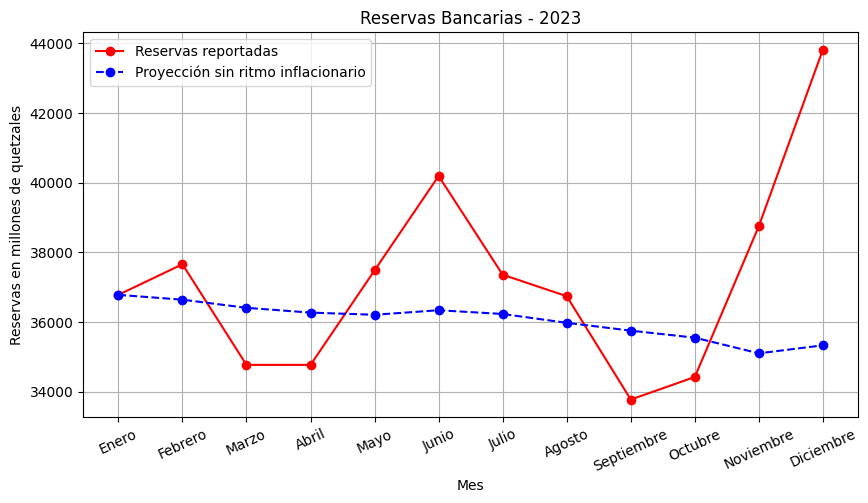
\includegraphics[width=\linewidth]{imagenes/retro_2023.png}
    \caption{2023}
  \end{subfigure}
\end{figure}


\subsection{Política Monetaria y Crediticia en Guatemala}
Guatemala ha implementado políticas monetarias y crediticias orientadas a fortalecer el sistema financiero y bancario  buscando adaptarse a estándares internacionales. Pondremos principal atención a la Resolución JM-47-2022, la cual se enfoca en actualizar el marco regulatorio para la valoración de activos. En la normativa, se establece un régimen de clasificación de activos y de reservas basado en la capacidad de pago y cumplimiento del deudor. Esta normativa busca gestionar el cumplimiento de reservas y la correcta gestión de riesgo de créditos. Esta normativa fue emitida por la Junta Monetaria de Guatemala el 25 de mayo de 2022, para entrar en vigencia a partir del 01 de enero de 2023. Claramente, esta política permite administrar mejor el riesgo en los bancos y respaldar el sistema financiero mediante la constitución de reservas bancarias. Sin embargo, como veremos más adelante, esto le exige a los bancos reservar cierto dinero que hasta antes de la política, no se reservaba, provocando así que las entidades bancarias se vean en la posición de ya sea aumentar tasas a los créditos o bien, mantener precios pero correr el riesgo de perder rentabilidad.

\subsubsection{JM-47-2022}
La Resolución JM-47-2022 introduce un marco regulatorio avanzado para la gestión del riesgo de crédito focalizándose en una metodología prospectiva para la evaluación de la capacidad de pago de los deudores y la adecuada clasificación de activos en función del riesgo. Técnicamente, esta normativa impone a los bancos el cálculo de provisiones basadas en la estimación de pérdidas esperadas, integrando conceptos como la Probabilidad de Incumplimiento (PI), la Pérdida Dado el Incumplimiento (PDI) y la Exposición al Momento del Incumplimiento (EMI), para refinar la estimación de reservas específicas y dinámicas. Específicamente, exige una valoración precisa de activos crediticios, incluyendo la alineación de activos crediticios bajo un enfoque de refinanciación y reestructuración, y la categorización de riesgos en activos según un modelo que contempla variables macroeconómicas y del mercado. A nivel operativo, los bancos deben, dependiendo del tipo de crédito y de la categoría del créditohabiente, reservar un porcentaje del monto del crédito que está otorgando. El lector puede consultar el Anexo \ref{categorias} para más información del cálculo de categorías. Puntualmente, los bancos deben calcular sus pérdidas esperadas, por el riesgo de crédito, con la fórmula
\begin{align}\label{formula pe}
    PE &= (PI) \times (PDI) \times (EMI).
\end{align}
Las probabilidades de incumplimiento son dadas en la Resolución de la normativa y se dividen entre probabilidades para créditos empresariales y créditos de productos, habiendo, posteriormente a esta división, una segmentación por tipo de crédito. El lector puede consultar el Anexo \ref{categorias} si desea ver algunas tablas de probabilidad de incumplimiento según tipo de crédito. Así mismo, la pérdida dado el incumplimiento se presenta según tipo de garantía del crédito y categoría del créditohabiente en el documento de la resolución. Se puede consultar la Resolución de la Normativa para más información.\footnote{El enlace a la resolución se encuentra en la bibliografía de este documento.} Finalmente, la exposición al momento de incumplimiento corresponde al saldo pendiente del crédito al momento del cálculo de las reservas. 

De esta forma, los bancos, con cada período de pago del crédito, deberán reservar un porcentaje de este de acuerdo a la probabilidad de incumplimiento y la pérdida dado el incumplimiento. Nótese que estos dos parámetros dependen del tipo y garantía del crédito y la categoría del créditohabiente. Además, la reserva, en quetzales, está dada por la fórmula \ref{formula pe}. 

\subsection{Desafíos actuales en la gestión del riesgo de crédito}
% aca hacer algun estudio de series de timepo para ver la estabilidad que se maneja actualmente y la esperada
% tambien se podria analizar la perspectiva de la jm47 en cuanto a garantizar reseras pero tambien cuidar a nivel micro a los creditohhabientes medinate un estudio de sus condiciones economicas

%vincular esto con el analisis de reservas e inflacion que se hizo antes

Con el nuevo paradigma de establecimiento de precios de crédito inducido por la JM47-2022, nos encontramos ante una situación que puede ser vista desde diferentes aristas.  Para analizar los desafíos actuales en la gestión del riesgo de crédito, iniciaremos revisando los datos de inflación y la formación de reservas, referenciados en los gráficos \ref{proyeccion reservas inicio de año} y \ref{proyeccion retro}. Aplicaremos un Modelo autorregresivo integrado de media móvil (ARIMA) para proyectar las reservas, conservando en el análisis tanto la curva de reservas iniciales del año como una proyección ajustada, excluyendo el efecto inflacionario. Esto nos permitirá evaluar cómo la acumulación de reservas se compara con las tendencias inflacionarias, brindando así una perspectiva cuantitativa sobre el asunto. Además, en el ámbito de las reservas bancarias, enfrentamos el reto de equilibrar la rentabilidad bancaria con la salud financiera de los créditohabientes. Por ende, el establecimiento de precios para el crédito no solo responde a criterios de rentabilidad y ganancia económica; representa también una cuestión de gran relevancia social y humana.

\subsubsection{Modelo autorregresivo integrado de media móvil: Análisis del desafío actual de Inflación y Reservas Bancarias}
Utilizando Python, ver anexo \ref{codigo sarima}, haremos una proyección de las reservas. Este estudio busca evaluar cuál sería el escenario futuro si se siguiera con la constitución de reservas bajo las normativas previas a la JM47-2022. La proyección se hará utilizando un Modelo SARIMA. Los parámetros no estacionarios utilizados para el modelo fueron $(p,d,q) = (1,1,1)$ y los  estacionarios, $(P,D, Q, S) = (0,0,2,12)$. Los parámetros fueron encontrados utilizando la librería estadística \textit{pmdarima} de Python. Los resultados de las proyecciones se muestran a continuación. 
\begin{figure}[H]
    \centering
    \begin{minipage}{.85\textwidth}
        \centering
        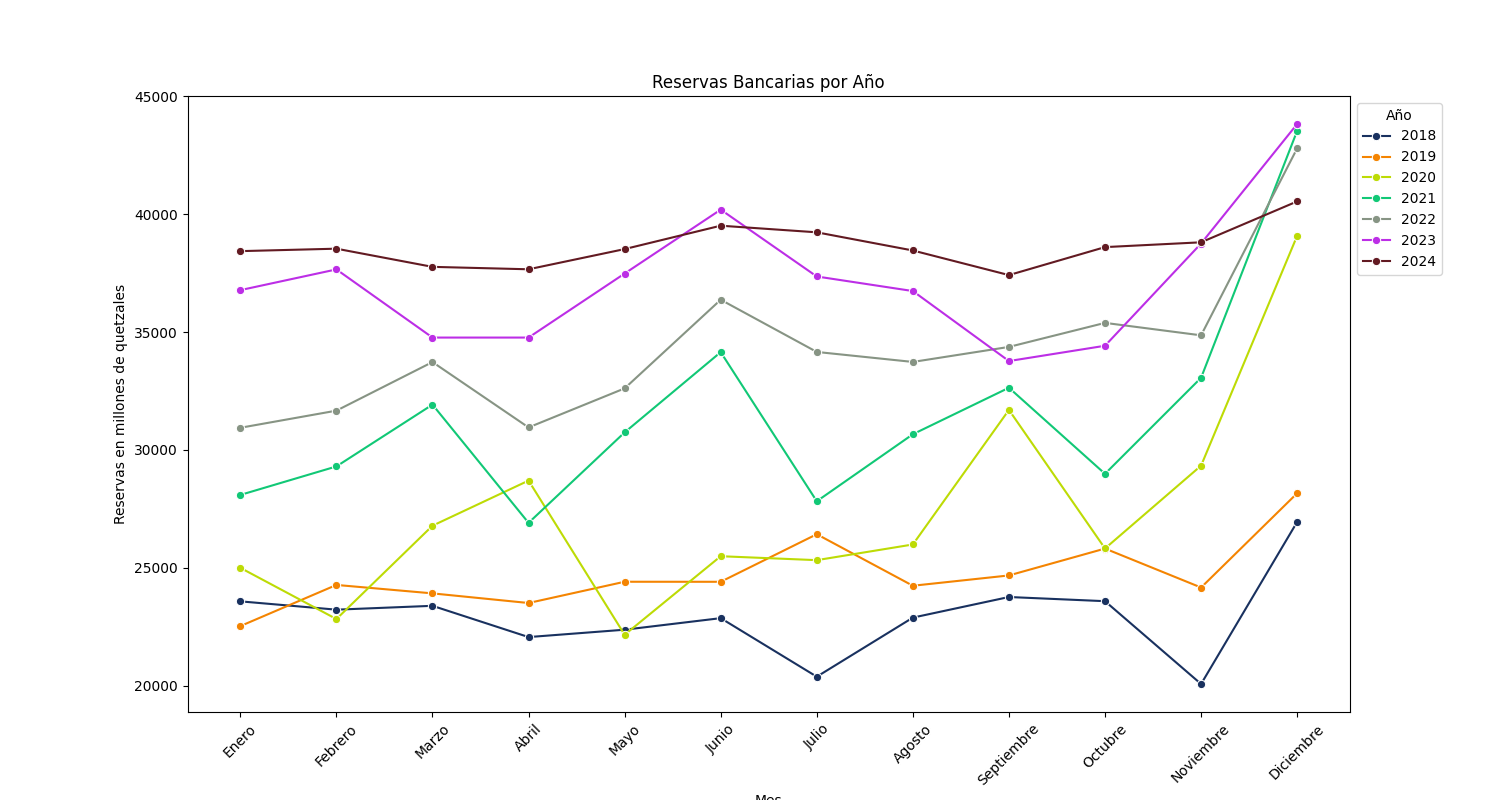
\includegraphics[width=\linewidth]{imagenes/prediccion_reservas_sarima.png}
        \caption{Predicción de las Reservas Bancarias 2024 usando modelo SARIMA}
        \label{fig:sarima-prediction}
    \end{minipage}%
    \begin{minipage}{.15\textwidth}
        \centering
        {\scriptsize 
        \begin{tabular}{lc}
            \hline
             & Valor (en quetzales) \\
            \hline
            MSE & 3,671,571.71 \\
            RMSE & 1,916.13 \\
            MAE & 1,558.97 \\
            AIC & 1,136.75 \\
            % BIC & 1,147.14 \\
            \hline
        \end{tabular}
        }
        %\captionof{table}{\scriptsize Nivel de error del modelo.}
        \label{proyeccion sarima}
    \end{minipage}
\end{figure}
En el gráfico referido como \ref{proyeccion sarima}, se observa que la proyección para las Reservas Bancarias al cierre de 2024 es inferior a las registradas en los años 2021, 2022 y 2023. A lo largo de 2024, sin embargo, las proyecciones sugieren que las Reservas podrían exceder los niveles de años anteriores. Cabe destacar que la tasa de acumulación de Reservas en diciembre de 2024 es menor comparada con la de diciembre de años previos, y la tendencia general de aumento y disminución de Reservas en 2024 muestra una curva más aplanada.

El propósito de este gráfico no es meramente comparativo o prescriptivo, sino que busca analizar la posible situación de las Reservas Bancarias bajo la continuación de las normativas actuales. Este análisis pretende resaltar la relevancia de mantener o ajustar la normativa vigente para reflejar las necesidades económicas. Aunque las metas de Reservas están influenciadas por diversos factores y objetivos económicos nacionales, un análisis más completo podría beneficiarse de incorporar factores adicionales, como la inflación. En términos generales, se puede concluir que, bajo el ritmo actual, las Reservas podrían resultar insuficientes al final del año, indicando la necesidad de modificar las directrices para su constitución. Además, para acelerar la formación de Reservas, alineándolo con los objetivos económicos del país, sería esencial mitigar el riesgo de crédito, posiblemente mediante el incremento de los requisitos para las reservas.
